\documentclass[varwidth=true, border=2pt]{standalone}

\usepackage{pgfplots}
\usepackage{tikz}

\usetikzlibrary{calc,patterns,angles,quotes}

\begin{document}
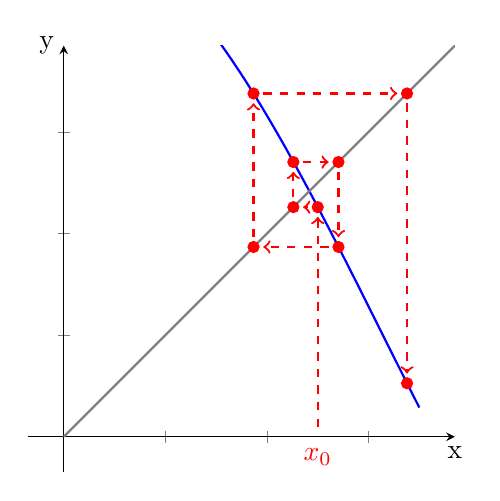
\begin{tikzpicture}
    \begin{axis}[
        legend pos=south east,
        axis x line=middle,
        axis y line=middle,
	every axis x label/.style={at={(current axis.right of origin)},anchor=north},
	every axis y label/.style={at={(current axis.above origin)},anchor=east},
	xticklabels=\empty,
	yticklabels=\empty
        grid = none ,
        width=7cm,
        height=7cm,
        grid style={dashed, gray!1},
        xmin=0,     % start the diagram at this x-coordinate
        xmax= 3.5,    % end   the diagram at this x-coordinate
        ymin=0,     % start the diagram at this y-coordinate
        ymax= 3.5,   % end   the diagram at this y-coordinate
        xlabel=x,
        ylabel=y,
        enlargelimits=true,
        tension=0.08]

        \addplot[domain=0:3.5,blue, thick,samples=250] {4*cos(deg(x/2))+1}; % Parabola
         \addplot[domain=-0:8, gray, thick,samples=250] {x};

	
	\node[red] (x0) at (axis cs: 2.5,0){};
	\node[red] (y0) at (axis cs: 2.5,2.26){};
	\node[red] (x1) at (axis cs: 2.26,2.26){};
	\node[red] (y1) at (axis cs: 2.26,2.704){};
	\node[red] (x2) at (axis cs: 2.704,2.704){};
	\node[red] (y2) at (axis cs: 2.704,1.868){};
	\node[red] (x3) at (axis cs: 1.868,1.868){};
	\node[red] (y3) at (axis cs: 1.868,3.379){};
	\node[red] (x4) at (axis cs: 3.379,3.379){};
	\node[red] (y4) at (axis cs: 3.379,0.526){};
	
	\node[red] (xL) at (axis cs: 2.5,-0.2){$x_0$};
	
	\draw[red, dashed, thick, ->](x0)--(y0);
	\draw[red, dashed, thick, ->](y0)--(x1);
	\draw[red, dashed, thick, ->](x1)--(y1);
	\draw[red, dashed, thick, ->](y1)--(x2);
	\draw[red, dashed, thick, ->](x2)--(y2);
	\draw[red, dashed, thick, ->](y2)--(x3);
	\draw[red, dashed, thick, ->](x3)--(y3);
	\draw[red, dashed, thick, ->](y3)--(x4);
	\draw[red, dashed, thick, ->](x4)--(y4);	
	
	
	\addplot[red, only marks, mark=*, mark size=2pt] coordinates {(2.5,2.26)(2.26,2.26)(2.26,2.704)(2.704,2.704)(2.704,1.868)(1.868,1.868)(1.868,3.379)(3.379,3.379)(3.379,0.526)};
	
    \end{axis}
\end{tikzpicture}
\end{document}